\documentclass[11pt,a4paper]{article}
\usepackage[T1]{fontenc}
\usepackage[utf8]{inputenc}
\usepackage[top=2.2cm, bottom=2.2cm, left=2.5cm, right=2.5cm]{geometry}
\usepackage{graphicx}
\usepackage{enumitem}
\usepackage{fancyvrb}
\usepackage{array}

\setlength{\parindent}{0pt}
\setlength{\parskip}{0.5em}
\linespread{1.08}

\setlist[itemize]{topsep=2pt, itemsep=3pt, parsep=0pt, leftmargin=1.5em}

\fvset{
    fontsize=\footnotesize,
    frame=single,
    framesep=5pt,
    samepage=false,
    xleftmargin=2pt,
    xrightmargin=2pt
}

\title{\textbf{Report.10.DB.Design.Magazine}\\[0.3em]\large Database Design Report -- Magazine Database}
\author{Tran Binh Minh \\ Student ID: 2640108}
\date{Information Systems (MI1.02a) \\ Labwork 05 -- Database design (exercise 1: magazine)}

\begin{document}
\maketitle

\section{The problem}
The goal is to keep track of the magazines I usually buy. Each magazine is described by its title, its ISSN (the code identifying the publication), its number and its year. The database must also hold the articles, each with a title, a first page and a last page; article titles are assumed to be unique. Several authors may contribute to one article. For every author the name, e-mail address and affiliation are recorded, together with a number giving that author's position in the author list of the article.

\section{How I made the structure}

\subsection{Conceptual model}
From the requirements, three entities stand out: magazines, articles and authors.
\begin{itemize}
    \item \textbf{Magazine}: ISSN, title, number and year. An ISSN identifies a publication as a whole rather than a single issue, so an issue is identified by the combination ISSN + number + year.
    \item \textbf{Article}: title, start page and end page. Because no title appears twice, the title alone can serve as the key.
    \item \textbf{Author}: name, e-mail and affiliation. The e-mail is used as the key, since different authors could share the same name.
\end{itemize}

Relationships:
\begin{itemize}
    \item An issue holds many articles, while every article appears in exactly one issue (one-to-many).
    \item An article may have several authors, and an author may write several articles (many-to-many). The author order is a property of this relationship itself, not of the article or of the author on their own.
\end{itemize}

\subsection{Logical model}
\begin{itemize}
    \item \texttt{Magazine(\underline{ISSN, Number, Year}, Title)} \\
    Primary key: \texttt{(ISSN, Number, Year)}
    \item \texttt{Article(\underline{ArticleTitle}, StartPage, EndPage, ISSN, Number, Year)} \\
    Primary key: \texttt{ArticleTitle}; Foreign key: \texttt{(ISSN, Number, Year)} $\rightarrow$ \texttt{Magazine}
    \item \texttt{Author(\underline{Email}, AuthorName, Affiliation)} \\
    Primary key: \texttt{Email}
    \item \texttt{Article\_author(\underline{ArticleTitle, Email}, AuthorOrder)} \\
    Primary key: \texttt{(ArticleTitle, Email)}; Foreign keys: \texttt{ArticleTitle} $\rightarrow$ \texttt{Article}, \texttt{Email} $\rightarrow$ \texttt{Author}
\end{itemize}

The many-to-many relationship is turned into a separate table, \texttt{Article\_author}, which is also where \texttt{AuthorOrder} lives.

Normalization: each column stores one atomic value, so all tables satisfy 1NF. Article, Author and Article\_author contain neither partial nor transitive dependencies. Magazine is the only exception: its title is determined by the ISSN alone, so the same title is repeated for every issue of a magazine. This was kept on purpose so the model stays close to the exercise statement; moving the title into a separate table keyed by ISSN would remove the redundancy.

\subsection{Physical model}
The ER diagram can be found in \texttt{Labwork-05a.png}. Names, titles and e-mails are stored as VARCHAR, while pages, numbers and years are INT. Every foreign key is declared with \texttt{ON UPDATE CASCADE} and \texttt{ON DELETE CASCADE}, meaning that removing an issue automatically removes its articles as well.

\IfFileExists{Labwork-05a.png}{%
    \begin{center}
        \vspace{0.3em}
        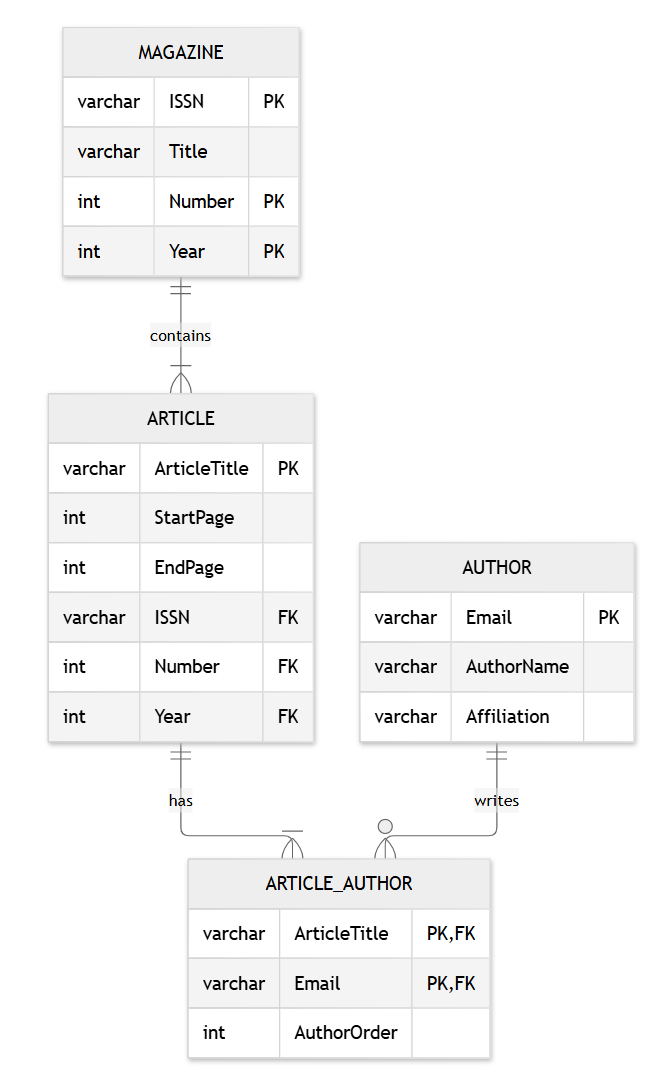
\includegraphics[width=0.85\textwidth, height=0.35\textheight, keepaspectratio]{Labwork-05a.png}
        \vspace{0.3em}
    \end{center}
}{}

\newpage
\section{SQL commands to create the database}
\begin{Verbatim}
DROP DATABASE IF EXISTS magazine_db;
CREATE DATABASE magazine_db;
USE magazine_db;

-- 1. Table: Magazine
CREATE TABLE MAGAZINE (
    ISSN VARCHAR(20) NOT NULL,
    Title VARCHAR(255) NOT NULL,
    Number INT NOT NULL,
    Year INT NOT NULL,
    PRIMARY KEY (ISSN, Number, Year)
);

-- 2. Table: Article
CREATE TABLE ARTICLE (
    ArticleTitle VARCHAR(255) NOT NULL,
    StartPage INT NOT NULL,
    EndPage INT NOT NULL,
    ISSN VARCHAR(20) NOT NULL,
    Number INT NOT NULL,
    Year INT NOT NULL,
    PRIMARY KEY (ArticleTitle),
    FOREIGN KEY (ISSN, Number, Year) REFERENCES MAGAZINE(ISSN, Number, Year)
        ON UPDATE CASCADE ON DELETE CASCADE
);

-- 3. Table: Author
CREATE TABLE AUTHOR (
    Email VARCHAR(255) NOT NULL,
    AuthorName VARCHAR(255) NOT NULL,
    Affiliation VARCHAR(255),
    PRIMARY KEY (Email)
);

-- 4. Table: Article_author
CREATE TABLE ARTICLE_AUTHOR (
    ArticleTitle VARCHAR(255) NOT NULL,
    Email VARCHAR(255) NOT NULL,
    AuthorOrder INT NOT NULL,
    PRIMARY KEY (ArticleTitle, Email),
    FOREIGN KEY (ArticleTitle) REFERENCES ARTICLE(ArticleTitle)
        ON UPDATE CASCADE ON DELETE CASCADE,
    FOREIGN KEY (Email) REFERENCES AUTHOR(Email)
        ON UPDATE CASCADE ON DELETE CASCADE
);
\end{Verbatim}

\newpage
\section{DESCRIBE commands and their outputs}
\begin{Verbatim}
-- DESCRIBE MAGAZINE;
+--------+--------------+------+-----+---------+-------+
| Field  | Type         | Null | Key | Default | Extra |
+--------+--------------+------+-----+---------+-------+
| ISSN   | varchar(20)  | NO   | PRI | NULL    |       |
| Title  | varchar(255) | NO   |     | NULL    |       |
| Number | int          | NO   | PRI | NULL    |       |
| Year   | int          | NO   | PRI | NULL    |       |
+--------+--------------+------+-----+---------+-------+

-- DESCRIBE ARTICLE;
+--------------+--------------+------+-----+---------+-------+
| Field        | Type         | Null | Key | Default | Extra |
+--------------+--------------+------+-----+---------+-------+
| ArticleTitle | varchar(255) | NO   | PRI | NULL    |       |
| StartPage    | int          | NO   |     | NULL    |       |
| EndPage      | int          | NO   |     | NULL    |       |
| ISSN         | varchar(20)  | NO   | MUL | NULL    |       |
| Number       | int          | NO   |     | NULL    |       |
| Year         | int          | NO   |     | NULL    |       |
+--------------+--------------+------+-----+---------+-------+

-- DESCRIBE AUTHOR;
+-------------+--------------+------+-----+---------+-------+
| Field       | Type         | Null | Key | Default | Extra |
+-------------+--------------+------+-----+---------+-------+
| Email       | varchar(255) | NO   | PRI | NULL    |       |
| AuthorName  | varchar(255) | NO   |     | NULL    |       |
| Affiliation | varchar(255) | YES  |     | NULL    |       |
+-------------+--------------+------+-----+---------+-------+

-- DESCRIBE ARTICLE_AUTHOR;
+--------------+--------------+------+-----+---------+-------+
| Field        | Type         | Null | Key | Default | Extra |
+--------------+--------------+------+-----+---------+-------+
| ArticleTitle | varchar(255) | NO   | PRI | NULL    |       |
| Email        | varchar(255) | NO   | PRI | NULL    |       |
| AuthorOrder  | int          | NO   |     | NULL    |       |
+--------------+--------------+------+-----+---------+-------+
\end{Verbatim}

\end{document}